\documentclass{article}

% Recommended, but optional, packages for figures and better typesetting:
\usepackage{microtype}
\usepackage{graphicx}
% \usepackage{subfigure}
\usepackage{caption}
\usepackage{subcaption}
\usepackage{booktabs} % for professional tables
\usepackage{kotex} %korean patch

% hyperref makes hyperlinks in the resulting PDF.
% If your build breaks (sometimes temporarily if a hyperlink spans a page)
% please comment out the following usepackage line and replace
% \usepackage{icml2019} with \usepackage[nohyperref]{icml2019} above.
\usepackage{hyperref}

% Attempt to make hyperref and algorithmic work together better:
\newcommand{\theHalgorithm}{\arabic{algorithm}}

% Use the following line for the initial blind version submitted for review:
%\usepackage{icml2019}

% If accepted, instead use the following line for the camera-ready submission:
\usepackage[accepted]{icml2019}

% The \icmltitle you define below is probably too long as a header.
% Therefore, a short form for the running title is supplied here:
\icmltitlerunning{COSE474-2023F: Final Project Proposal}

\begin{document}

\twocolumn[
\icmltitle{COSE474-2021F: Final Project Proposal \\
           optimizer 가능성 탐구}

% It is OKAY to include author information, even for blind
% submissions: the style file will automatically remove it for you
% unless you've provided the [accepted] option to the icml2019
% package.

% List of affiliations: The first argument should be a (short)
% identifier you will use later to specify author affiliations
% Academic affiliations should list Department, University, City, Region, Country
% Industry affiliations should list Company, City, Region, Country

% You can specify symbols, otherwise they are numbered in order.
% Ideally, you should not use this facility. Affiliations will be numbered
% in order of appearance and this is the preferred way.
\icmlsetsymbol{equal}{*}

\begin{icmlauthorlist}
\icmlauthor{2019320138 김규진}{}
\end{icmlauthorlist}

%\icmlaffiliation{ku}{Department of Computer Science \& Engineering, Korea University, Seoul, Korea}


%\icmlcorrespondingauthor{the}{myemail@korea.ac.kr}
%\icmlcorrespondingauthor{Eee Pppp}{ep@eden.co.uk}

% You may provide any keywords that you
% find helpful for describing your paper; these are used to populate
% the "keywords" metadata in the PDF but will not be shown in the document
\icmlkeywords{Machine Learning, ICML}

\vskip 0.3in
]

% this must go after the closing bracket ] following \twocolumn[ ...

% This command actually creates the footnote in the first column
% listing the affiliations and the copyright notice.
% The command takes one argument, which is text to display at the start of the footnote.
% The \icmlEqualContribution command is standard text for equal contribution.
% Remove it (just {}) if you do not need this facility.

%\printAffiliationsAndNotice{}  % leave blank if no need to mention equal contribution
%\printAffiliationsAndNotice{\icmlEqualContribution} % otherwise use the standard text.

%\begin{abstract}
%This document provides a basic paper template and submission guidelines.
%Abstracts must be a single paragraph, ideally between 4--6 sentences long.
%Gross violations will trigger corrections at the camera-ready phase.
%\end{abstract}

\section{Introduction}
딥러닝 과정에서 설정하고 연결해줘야 할 모듈들로는 activation function, normalize, regularize 등 다양한 기초적인 모듈들이 있다. 이런 기본적인 모듈에서도 다양한 방식이 활용되고 있으며, 학습하는 모델에 따라 각 dataset에 따라 어떤 방식을 활용하는 지에 따라 그 학습의 결과 또한 최적의 결과를 낼 수도, 내지 못 할 수도 있다. 때문에 적절한 모듈을 선택하는 것이 가장 중요하다고 할 수 있다.\\
이 중에서도 이번 연구에서 주목하게 된 부분은 optimizer 모듈을 만드는 부분이다. Optimizer가 잘 선택된다면 optimize된 결과가 나올 때 까지 반복 작업해야하는 epoch의 수를 줄일 수 있기 때문에, 결과가 나오기까지의 computing power를 획기적으로 줄일 수 있다. 이를 통해 우리는 결과 도출까지의 시간을 줄이거나, 같은 시간 안에 더 질 좋은 결과를 산출할 수 있게 될 것이다.\\
Optimizer로 가장 대표적으로 사용된다고 할 수 있는 것은 바로 Momentum optimizer이다. 이름에서도 볼 수 있듯 관성 개념을 학습에 적용시켜 gradient descending 작업을 단축시키는 방식인데, 이처럼 다양한 optimizer를 만들어내는 데 있어서 나름의 철학과 현상을 가지고 optimizer의 기능을 구현하고 있다. 이러한 생각에서 영감을 받아, 이번 연구에서는 현실에 있는 여러 개념을 이용해 새로운 optimizer들을 고안해 만들어보고자 했다.\\
또, 여러 optimizer에서는 learning rate를 선형적으로 곱해해주는 방식을 활용하고 있는데, 이에 비선형적으로 적용하는 방식은 왜 주목되지 못하는지에 대해서도 함께 알아보고자 한다.\\
해당 연구에서는 Base가 되는 모델로는 momentum optimizer을 이용했다. 관성을 이용하는 가장 기본적인 모델이기도 하며, 다양한 optimizer가 momentum optimizer에서 파생해 만들어졌기 때문에 선택하게 되었다. momentum optimizer과는 구분되는 차별점은 크게 두가지이다. 따로 scheduling을 설정해 학습을 진행하는 타 의례와는 달리, learning rate를 연산 과정에서 비선형적으로 설계해 차별점을 만들었다. 또, 학습 가속에 있어 중력의 개념과 학습 방향에 있어 새로운 개념을 도입함으로써 연산 과정에서 비선형적으로 상황에 맞는 학습 강도가 설정될 수 있도록 함으로써 optimizer에 새로운 방향을 제시했다. 이런 방법을 활용한다면 가상의 기대되는 적절한 값과는 차이가 있는 learning rate를 이용했더라도 optimizer가 타협하여 learning rate를 조절하는 기대효과를 낼 수 있다. 이를 통해 더 적은 epoch를 이용해 같은 결과를 더 빠르게 도출해낼 수 있을 것이라고 예상하고 실험을 진행했다.\\


\section{Methods}
여기서는 optimizer을 만드는 데 있어 새로운 개념을 도입한 두 가지 새로운 optimizer을 이용한다. 이 두 가지는 learning rate를 결과값을 향한 중력 방식의 가속도의 강도라는 개념을 도입한 gravity optimizer와, momentum이 가리키는 방향과 진행방향이 다르다면 급격한 가중치를 주어 방향을 전환시키는 cosine optimizer을 소개한다.\\
1. gravity optimizer\\
첫 번째 소개할 방식은 gravity optimizer이다. 이는 기본적인 weight의 방향 말고, 결과값을 향한 가속도를 lr의 크기로 설정한다. 이를 통해 벡터가 클수록 더 강한 속도로 학습되고 있음을 보정한다. Algorithm~\ref{alg:gravity} 이 그 의사코드 형태를 보여준다. \\
우선 Figure~\ref{prf:cosine}을 보면, 유도 과정을 쉽게 이해할 수 있다. 결과부터 이야기를 하자면, 원래의 gradient값을 가지는 gradient vector에서 gravity만큼의 방향벡터를 추가해 cosine vector와 같은 크기로 조정을 해주는 것이다. 먼저 gradient vector는 gradient로 이루어진 전체 vector의 크기이다. gravity가 사실상 핵심 부분이다. gravity는 $lr\cdot\sqrt{N}$으로, learning rate를 vector dimension의 루트로 나눈 것으로 한다. 그냥 lr로 할 수 있지만 $\sqrt{N}$으로 곱해준 것은 demension이 너무 커질 경우, 아무리 lr을 값을 조정해도 그 사이즈 때문에 의미가 없는 값처럼 작아지기 때문이다. 그렇기 때문에 $\sqrt{N}$를 곱해 의미가 있도록 해준다. 이후 계산이 중요하다. \\
$\vec{cosine}=\sqrt{(\vec{gradient})^2+gravity^2} \\
cos\theta=\frac{|\vec{gradient|}}{|\vec{cosine}|} \\
\vec{newgradient}=\vec{gradient}*cos\theta $ \\
이렇게 gradient를 새로 조정하게 되면 learning rate를 gravity로 적용할 수 있다. 이를 momentum 알고리즘에 적용해 만든 gravity momentum optimizer가 Algorithm~\ref{alg:gravity}에 작성되어있다.

\begin{figure}
   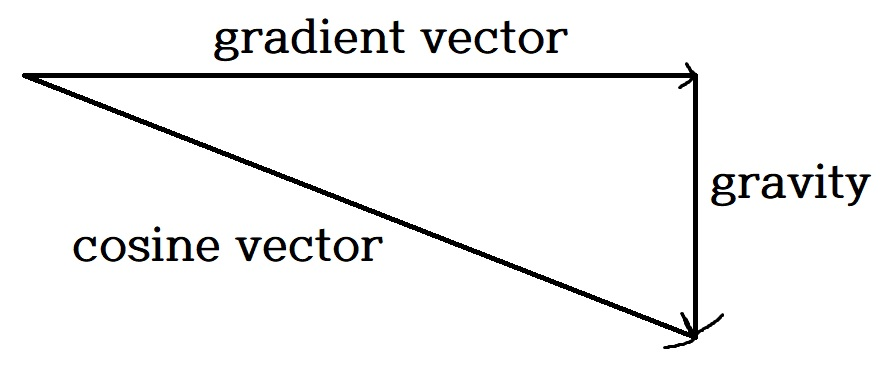
\includegraphics[width=\columnwidth]{img/cosine vector.jpg}
   \caption{Gravity Momentum}
   \label{prf:cosine}
\end{figure}

\begin{algorithm}[tb]
   \caption{Gravity Optimizer}
   \label{alg:gravity}
\begin{algorithmic}
   \STATE {\bfseries Input:} parameter matrix array $params$, gradient matrix array $grad$, saver matrix array $m$, learning rate $lr$, parameter dimension $N$, momentum rate $u$
   \REPEAT
   \STATE for param in params
   \FOR {$param$ {\bfseries in} $params$}
   \STATE $S=\sum{\frac{(grad)^2}{N}}$
   \STATE $k=\sqrt{1+\frac{lr^2}{S}}$
   \STATE $m=um-k\cdot lr\cdot grad$
   \STATE $param+=m$
   \ENDFOR
   \UNTIL{backpropagations are finished}
\end{algorithmic}
\end{algorithm}

2. cosine optimizer\\
두 번째 소개할 방식은 cosine optimizer이다. 이는 현재 진행방향이 이번에 받은 가속도와 방향이 많이 다를수록, 더 확실하게 이번 가속도를 많이 반영하는 방식이다. 말 그대로 두 벡터의 회전각을 구해 각이 평각에 가까워질수록 더 작은 값을 적용하도록 한다.\\$cos\theta=\frac{\vec{m}\cdot\vec{g}}{||m||\cdot||g||}$를 통해 각도를 구한 후, 저장되어있는 과거의 momentum에 추가해준다. 각이 벌어질수록 0에 가깝고 각이 작을수록 그대로 해줘야하니 값을 변형해 적용한다. Algorithm~\ref{alg:cosine}에서 의사코드 형태를 보인다.

\begin{algorithm}[tb]
   \caption{Cosine Optimizer}
   \label{alg:cosine}
\begin{algorithmic}
   \STATE {\bfseries Input:} parameter matrix array $params$, gradient matrix array $grad$, saver matrix array $m$, cosine value matrix array $cosine$, cosine constant $C$, learning rate $lr$
   \REPEAT
   \FOR {$param$ {\bfseries in} $params$}
   \FOR {$\vec{m}, \vec{g}, \vec{cos}$ {\bfseries in} $m, gradient, cosine$}
   \STATE $cos\theta=\frac{\vec{m}\cdot\vec{g}}{||m||\cdot||g||}$
   \STATE $\vec{cos}=cos\theta\cdot\vec{1}$
   \ENDFOR
   \STATE $m=C \frac{cosine+1}{2}m+lr\cdot gradient$
   \STATE $param-=m$
   \ENDFOR
   \UNTIL{backpropagations are finished}
\end{algorithmic}
\end{algorithm}

두가지 방식이 모두 효과적인 향상을 불러일으키지 못하더라도 optimizer을 실제로 구현해보며 optmizer에 대한 개인적 이해를 높일 수 있고, optimizer가 요구하는 사항이 어떤 것이 있는지 더 자세하게 알아볼 수 있을 것이다.
plateau현상과 zigzag가 가장 optimizer의 과제이다. 이를 위해 Momentum방식을 이용했지만, 이는 zigzag 문제를 해결해주지 못했기에 adaptive방식과 혼합된 adam이 주로 사용되는 추세이다. nesterov momentum 방식은 비용에 비해 성능 향상이 적었다고 한다. 이에 많은 optimizer들 중 momentum optimizer을 이용한 결과와 비교하여 성능향상이 실제로 일어났는지 비교하고자 한다.

\section{Experiments}
% - Dataset
데이터셋은 튜토리얼에서 진행한 옷을 이용한 FashionMNIST dataset을 이용했다. 28*28개의 옷 이미지를 한 이미지로 하여 70,000개의 데이터가 있다. 10개의 카테고리로 분류되어있으며, training set과 validation set으로는 6:1로 나누고 있다.
% - Computing resource (CPU,GPU, OS, pytorch etc.)
computing resource는 dataset의 규모가 크지 않기에 CPU를 이용한다. windows 10 환경에서 실행했으며, pytorch를 활용해 코드를 작성한다.
% - Experimental design/setup
환경이 되는 터미널은 python 3.10.4를 이용했으며, ipynb 확장자로 작업해 작성되었다. 이미지가 한 장 당 28*28개로 784개이므로 input을 784로 잡았으며, category 수가 10개 이므로 output을 10개로 설정했다. momentum rate는 0.03로 최종 설정 한 후 learning rate를 0.2, 0.1, 0.05, 0.01로 차츰 변경해가며 테스트를 진행했다. 전체 epoch 수는 50개로 늘려 더 많은 학습이 진행되도록 변경했다.
% - Quantitative results / comparison with baselines, SOTA
SOTA는 momentum optimizer로 딥러닝을 실행했을 때의 결과를 Default result로 잡았다. 높은 learning rate에서는 gravity optimizer에서 overflow가 나고, 다른 여러 learning rate 환경에서 테스트한 작업들에 대해서는 큰 성능 향상을 확인할 수는 없었지만, learning rate를 0.05로 설정하고 진행된 실험에서는 눈에 띄는 변화를 확인할 수 있었다. Figure~\ref{lr:0.05}에서 gravity optimizer로 진행한 두번째 실험에서는 training loss와 validation loss가 1.8배 빠르게 감소하는 모습을 확인할 수 있다. 실행시간 또한 momentum optimizer를 실행했을 때와 거의 동일한 시간 안에 작동하는 모습을 보이며 상당한 효과를 보여줬다. 하지만, cosine optimizer과 같은 경우는 Figure~\ref{lr:0.2}에서 확인할 수 있듯 epoch 10~20 사이에서 oscillation을 조금 줄였을 뿐, 성능 향상에 있어 두각을 나타내지 못했다. 오히려, 타 optimizer과는 대비해 실행시간이 2배 가량 많이 걸리는 모습을 확인할 수 있다.
% - Figures (plots)/Tables and their analysis

\begin{figure}[ht]
\begin{center}\centering
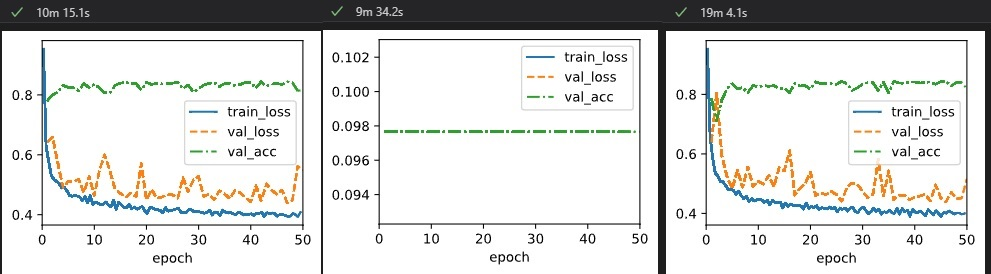
\includegraphics[width=\columnwidth]{img/lr0.2 m0.03.jpg}
\caption{lr=0.2}
\label{lr:0.2}
\end{center}
\end{figure}

\begin{figure}
\centering
   \begin{subfigure}{0.3\columnwidth}
      \centering
      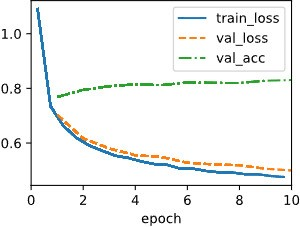
\includegraphics[width=\columnwidth]{img/lr0.1 sgd.jpg}
      \caption{sgd}
   \end{subfigure}
   \hfill
   \begin{subfigure}[b]{0.3\columnwidth}
      \centering
      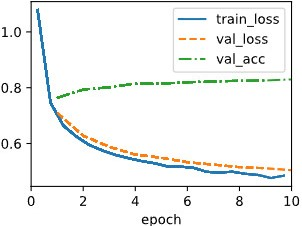
\includegraphics[width=\columnwidth]{img/lr0.1 gravity.jpg}
      \caption{gravity}
   \end{subfigure}
   \hfill
   \begin{subfigure}[b]{0.3\columnwidth}
      \centering
      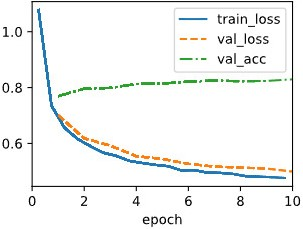
\includegraphics[width=\columnwidth]{img/lr0.1 cosine.jpg}
      \caption{cosine}
   \end{subfigure}
\caption{lr=0.1}
\label{lr:0.1}
\end{figure}

\begin{figure}
   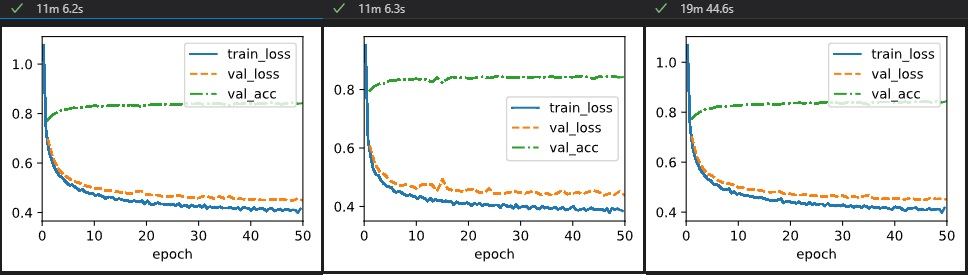
\includegraphics[width=\columnwidth]{img/lr0.05 m0.03.jpg}
\caption{lr=0.05}
\label{lr:0.05}
\end{figure}

\begin{figure}[ht]
\begin{center}\centering
\begin{subfigure}[b]{0.3\columnwidth}\centering
   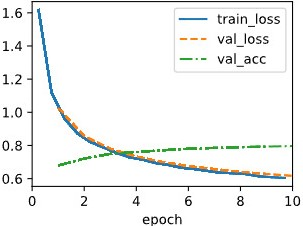
\includegraphics[width=\columnwidth]{img/lr0.01 sgd.jpg}
\end{subfigure}
\hfill
\begin{subfigure}[b]{0.3\columnwidth}\centering
   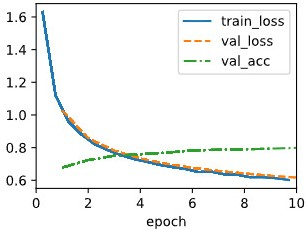
\includegraphics[width=\columnwidth]{img/lr0.01 gravity.jpg}
\end{subfigure}
\hfill
\begin{subfigure}[b]{0.3\columnwidth}\centering
   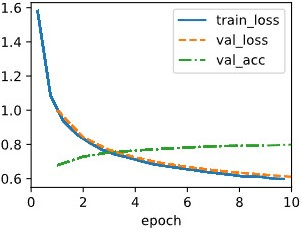
\includegraphics[width=\columnwidth]{img/lr0.01 cosine0.1.jpg}
\end{subfigure}
\hfill
\begin{subfigure}[b]{0.3\columnwidth}\centering
   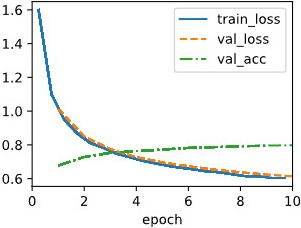
\includegraphics[width=\columnwidth]{img/lr0.01 cosine0.05.jpg}
\end{subfigure}
\hfill
\begin{subfigure}[b]{0.3\columnwidth}\centering
   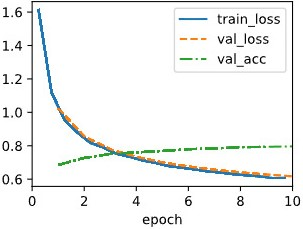
\includegraphics[width=\columnwidth]{img/lr0.01 cosine0.01.jpg}
\end{subfigure}
\caption{lr=0.01}
\label{lr:0.01}
\end{center}
\end{figure}

% - Discussion why the proposed method is successful or unsuccessful 
왜 gravity optimizer가 성능 향상이 발생했는지는 명확하다. gradient값을 연산해 learning rate를 조금 더 유연하게 증가시켜줬으므로 속도가 빨라진다. 추가적인 연산이 발생하지만, 거의 선형적인 연산이기 때문에 추가적인 시간이 전체 연산에 비해 큰 연산이 아니라서 시간 마저도 크게 차이나지 않는다.
cosine optimizer가 실패한 데에 있어서는 분석에 있어 어려움이 있었다. 일단 cosine optimizer을 코드로 구현하는 과정에 있어 vector를 input 784개를 한개의 vector로 구성하는 식으로 진행했어야 하는데, output 10개를 vector로 구성하는 식으로 코드가 짜여진 것을 보인다. 때문에 정확한 vector를 이용하지 않아 큰 차이가 발생했다. 또, vector의 방향이 맞지 않으면 빠르게 방향을 전환하는 방식을 이용하고 있는데, 여기 있어서도 문제점이 발생한다. 방향은 분명 빠르게 전환하지만, 그 과정에서 현재까지 가지고 있던 momentum을 전부 잃게 된다. 또, 각이 벌어지는 것을 통한 조정이 오히려 learning rate가 비교적 작은 쪽에서는 크게 영향을 주지 못한다. 오히려 learning rate를 0.2로 매우 과하게 잡은 곳에서 momentum optimizer이나 gravity optimizer보다 조금 더 나은 결과를 보여주는 것을 Figure~\ref{lr:0.2}에서 확인할 수 있다.\\
가장 결정적인 문제로는, 작은 dataset size를 들 수 있다. input 784개와 batch size 256개로 연산을 해도 epoch가 10개 정도로 거의 결론이 나오는 데이터셋을 가지고 50까지 돌리며 작업을 했기 때문에 어느정도 차이가 발생하는 것을 겨우 확인할 수 있었다. 이는 dataset의 규모가 비교적으로 너무 작은 것을 활용했기 때문에 결과 차이를 더 비교하지 못했을 것이라고 예상된다.

\section{Future direction}
다음에는 다른 데이터셋을 활용해 훨씬 대규모의 데이터를 처리해 봐야할 것이다. epoch가 100은 되는 것을 해봐야하지 않을까?
classification을 활용하는 것은 그대로 가는 것이 좋을 것 같다.

\bibliography{example_paper}
\bibliographystyle{icml2019}
\clearpage



\end{document}
